\begin{bt}%[9D6H18-2]
% nguon: Đề tham khảo Tuyển sinh 10 TP.HCM 2025-2026 – Huyện Cần Giờ (Đề 2), Bài 1, trang 93
Cho parabol $(P): y = x^2$.
\begin{enumerate}[a)]
	\item Vẽ đồ thị $(P)$ trên mặt phẳng tọa độ $Oxy$.
	\item Tìm tọa độ các điểm thuộc $(P)$ có tung độ bằng $9$.
\end{enumerate}
\loigiai{
	\begin{enumerate}[a)]
		\item Bảng giá trị tương ứng giữa $x$ và $y$:
		\begin{center}
		\begin{tabular}{|c|c|c|c|c|c|}
		\hline
		$x$ & $-2$ & $-1$ & $0$ & $1$ & $2$ \\
		\hline
		$y = x^2$ & $4$ & $1$ & $0$ & $1$ & $4$ \\
		\hline
		\end{tabular}
		\end{center}
		Đồ thị $(P)$ là đường cong parabol đi qua các điểm $(-2; 4)$, $(-1; 1)$, $(0; 0)$, $(1; 1)$, $(2; 4)$, nhận trục tung làm trục đối xứng và có đỉnh là gốc tọa độ $O(0; 0)$.
		\begin{center}
		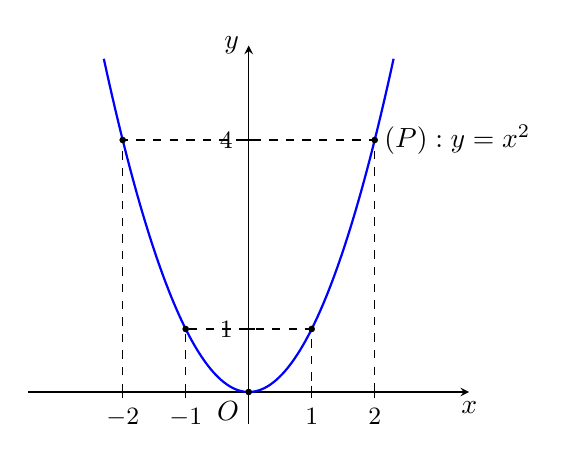
\begin{tikzpicture}[>=stealth, scale=0.8]
			\draw[->] (-3.5,0) -- (3.5,0) node[below] {$x$};
			\draw[->] (0,-0.5) -- (0,5.5) node[left] {$y$};
			\draw (0,0) node[below left] {$O$};
			\foreach \x in {-2,-1,1,2}
				\draw (\x,0.1) -- (\x,-0.1) node[below] {\small $\x$};
			\foreach \y in {1,4}
				\draw (0.1,\y) -- (-0.1,\y) node[left] {\small $\y$};
			\draw[dashed] (-2,0) -- (-2,4) -- (2,4) -- (2,0);
			\draw[dashed] (-1,0) -- (-1,1) -- (1,1) -- (1,0);
			\draw[smooth,samples=100,domain=-2.3:2.3,thick,blue] plot(\x,{(\x)^2});
			\node[right] at (2,4) {$(P): y=x^2$};
			\fill (-2,4) circle (1.5pt) (-1,1) circle (1.5pt) (0,0) circle (1.5pt) (1,1) circle (1.5pt) (2,4) circle (1.5pt);
		\end{tikzpicture}
		\end{center}
		\item Gọi điểm cần tìm là $M(x; y) \in (P)$.
		Theo đề bài, tung độ của điểm đó bằng $9$, tức là $y = 9$.
		Thay $y = 9$ vào phương trình parabol $(P)$, ta có:
		$$x^2 = 9 \iff x = 3 \text{ hoặc } x = -3.$$
		Vậy có hai điểm thuộc $(P)$ có tung độ bằng $9$ là $(3; 9)$ và $(-3; 9)$.
	\end{enumerate}
}
\end{bt}

\begin{bt}%[9D6H20-2]
% nguon: Đề tham khảo Tuyển sinh 10 TP.HCM 2025-2026 – Huyện Cần Giờ (Đề 2), Bài 2, trang 93
Cho phương trình bậc hai: $3x^2 - 12x + 2 = 0$.
\begin{enumerate}[a)]
	\item Chứng minh phương trình luôn có hai nghiệm phân biệt $x_1, x_2$.
	\item Không giải phương trình, hãy tính giá trị của biểu thức:
	$$A = \frac{x_1}{x_2 - 1} + \frac{x_2}{x_1 - 1}$$
\end{enumerate}
\loigiai{
	\begin{enumerate}[a)]
		\item Xét phương trình $3x^2 - 12x + 2 = 0$ có các hệ số $a = 3$, $b' = -6$, $c = 2$.
		Ta có:
		$$\Delta' = (b')^2 - ac = (-6)^2 - 3 \cdot 2 = 36 - 6 = 30 > 0.$$
		Vì $\Delta' > 0$ nên phương trình luôn có hai nghiệm phân biệt $x_1, x_2$.
		\item Theo định lý Vi-ét, ta có:
		$$\begin{cases} x_1 + x_2 = -\dfrac{b}{a} = -\dfrac{-12}{3} = 4 \\ x_1 x_2 = \dfrac{c}{a} = \dfrac{2}{3} \end{cases}$$
		Quy đồng mẫu thức biểu thức $A$:
		\begin{align*}
		A &= \frac{x_1(x_1 - 1) + x_2(x_2 - 1)}{(x_2 - 1)(x_1 - 1)} \\
		  &= \frac{x_1^2 - x_1 + x_2^2 - x_2}{x_1 x_2 - (x_1 + x_2) + 1} \\
		  &= \frac{(x_1 + x_2)^2 - 2x_1 x_2 - (x_1 + x_2)}{x_1 x_2 - (x_1 + x_2) + 1}
		\end{align*}
		Thay $x_1 + x_2 = 4$ và $x_1 x_2 = \dfrac{2}{3}$ vào biểu thức $A$, ta được:
		$$A = \frac{4^2 - 2 \cdot \dfrac{2}{3} - 4}{\dfrac{2}{3} - 4 + 1} = \frac{16 - \dfrac{4}{3} - 4}{\dfrac{2}{3} - 3} = \frac{12 - \dfrac{4}{3}}{-\dfrac{7}{3}} = \frac{\dfrac{32}{3}}{-\dfrac{7}{3}} = -\frac{32}{7}.$$
		Vậy $A = -\dfrac{32}{7}$.
	\end{enumerate}
}
\end{bt}

\begin{bt}%[9D6V21-3]
% nguon: Đề tham khảo Tuyển sinh 10 TP.HCM 2025-2026 – Huyện Cần Giờ (Đề 2), Bài 3, trang 93
Một mảnh đất hình chữ nhật có kích thước $8\text{ m} \times 20\text{ m}$. Để phục vụ việc mở rộng đường giao thông nông thôn, Nhà nước thu hồi một phần đất phía trước có dạng hình tam giác vuông với độ dài hai cạnh góc vuông lần lượt là $2x\text{ (m)}$ và $x\text{ (m)}$ ($0 < x < 8$).
\begin{enumerate}[a)]
	\item Viết công thức tính diện tích $T(x)\text{ (m}^2\text{)}$ phần đất bị thu hồi theo $x$.
	\item Biết tổng số tiền gia đình nhận được từ việc đền bù giải tỏa là $455$ triệu đồng và đơn giá đền bù là $13$ triệu đồng/$\text{m}^2$. Hãy tính độ dài cạnh $x$ (làm tròn kết quả đến hàng phần trăm).
\end{enumerate}
\loigiai{
	\begin{enumerate}[a)]
		\item Phần đất bị thu hồi có dạng tam giác vuông với hai cạnh góc vuông có độ dài $2x\text{ (m)}$ và $x\text{ (m)}$.
		Diện tích phần đất bị thu hồi là:
		$$T(x) = \frac{1}{2} \cdot 2x \cdot x = x^2\text{ (m}^2\text{)}.$$
		\item Diện tích đất được đền bù là:
		$$T(x) = \frac{455}{13} = 35\text{ (m}^2\text{)}.$$
		Theo câu a, ta có phương trình:
		$$x^2 = 35.$$
		Vì $x > 0$ nên:
		$$x = \sqrt{35} \approx 5{,}92\text{ (m)}.$$
		Giá trị này thỏa mãn điều kiện $0 < x < 8$.
		Vậy độ dài cạnh $x$ xấp xỉ bằng $5{,}92\text{ m}$.
	\end{enumerate}
}
\end{bt}

\begin{bt}%[9H0V31-3]
% nguon: Đề tham khảo Tuyển sinh 10 TP.HCM 2025-2026 – Huyện Cần Giờ (Đề 2), Bài 4, trang 93
Một cái ao sâu có dạng nửa hình cầu với đường kính $10\text{ m}$. Người ta dùng xe tải để chở đất đến san lấp toàn bộ ao nước này.
\begin{enumerate}[a)]
	\item Tính thể tích nước chứa trong ao khi đầy nước (biết công thức thể tích hình cầu là $V = \dfrac{4}{3}\pi R^3$, lấy $\pi \approx 3{,}14$ và làm tròn kết quả đến chữ số thập phân thứ nhất).
	\item Thùng xe tải có dạng hình hộp chữ nhật với kích thước dài $9{,}9\text{ m}$, rộng $2{,}37\text{ m}$ và cao $0{,}85\text{ m}$. Mỗi chuyến xe chỉ được phép chở tối đa $85\%$ thể tích của thùng xe để đảm bảo an toàn giao thông. Hỏi cần ít nhất bao nhiêu chuyến xe tải chở đất như vậy để có thể san lấp đầy cái ao trên?
\end{enumerate}
\loigiai{
	\begin{enumerate}[a)]
		\item Bán kính của ao dạng nửa hình cầu là:
		$$R = \frac{10}{2} = 5\text{ (m)}.$$
		Thể tích nước chứa đầy trong ao là:
		$$V = \frac{1}{2} \cdot \left(\frac{4}{3}\pi R^3\right) = \frac{2}{3} \cdot 3{,}14 \cdot 5^3 = \frac{785}{3} \approx 261{,}7\text{ (m}^3\text{)}.$$
		\item Thể tích của thùng xe tải hình hộp chữ nhật là:
		$$V_{\text{thùng}} = 9{,}9 \cdot 2{,}37 \cdot 0{,}85 = 19{,}94355\text{ (m}^3\text{)}.$$
		Lượng đất tối đa mỗi chuyến xe được phép chở là:
		$$V_{\text{chở}} = 85\% \cdot V_{\text{thùng}} = 0{,}85 \cdot 19{,}94355 = 16{,}9520175\text{ (m}^3\text{)}.$$
		Số chuyến xe ít nhất cần để chở đất san lấp đầy ao là:
		$$\frac{V}{V_{\text{chở}}} = \frac{261{,}7}{16{,}9520175} \approx 15{,}44\text{ (chuyến)}.$$
		Vì số chuyến xe phải là số nguyên nên cần ít nhất $16$ chuyến xe tải.
	\end{enumerate}
}
\end{bt}

\begin{bt}%[9D1H3-4]
% nguon: Đề tham khảo Tuyển sinh 10 TP.HCM 2025-2026 – Huyện Cần Giờ (Đề 2), Bài 5, trang 94
Có ba bình đựng nước với tổng thể tích là $132$ lít. Người ta rót nước từ bình thứ nhất đang đầy sang hai bình kia:
\begin{itemize}
	\item Nếu đổ đầy bình thứ ba thì bình thứ hai chỉ được thêm một nửa lượng nước so với dung tích của nó.
	\item Nếu đổ đầy bình thứ hai thì bình thứ ba chỉ được thêm một phần ba lượng nước so với dung tích của nó.
\end{itemize}
Hỏi dung tích của mỗi bình là bao nhiêu lít?
\loigiai{
	Gọi dung tích của bình thứ nhất, bình thứ hai, bình thứ ba lần lượt là $x, y, z$ (lít) ($x, y, z > 0$).\\
	Tổng dung tích của ba bình là $132$ lít, ta có phương trình:
	$$x + y + z = 132 \quad (1)$$
	Theo đề bài, lượng nước có trong bình thứ nhất đang đầy là $x$ lít.\\
	Khi rót nước từ bình thứ nhất:
	\begin{itemize}
		\item Đổ đầy bình thứ ba (cần $z$ lít) thì bình thứ hai được một nửa dung tích của nó (là $\dfrac{1}{2}y$ lít), ta có:
		$$x = z + \frac{1}{2}y \quad (2)$$
		\item Đổ đầy bình thứ hai (cần $y$ lít) thì bình thứ ba được một phần ba dung tích của nó (là $\dfrac{1}{3}z$ lít), ta có:
		$$x = y + \frac{1}{3}z \quad (3)$$
	\end{itemize}
	Từ $(2)$ và $(3)$, suy ra:
	$$z + \frac{1}{2}y = y + \frac{1}{3}z \iff \frac{2}{3}z = \frac{1}{2}y \iff y = \frac{4}{3}z.$$
	Thay $y = \dfrac{4}{3}z$ vào $(2)$, ta được:
	$$x = z + \frac{1}{2} \cdot \left(\frac{4}{3}z\right) = z + \frac{2}{3}z = \frac{5}{3}z.$$
	Thay $x = \dfrac{5}{3}z$ và $y = \dfrac{4}{3}z$ vào $(1)$, ta được:
	$$\frac{5}{3}z + \frac{4}{3}z + z = 132 \iff 4z = 132 \iff z = 33\text{ (thỏa mãn)}.$$
	Từ đó tính được:
	\begin{align*}
	y &= \frac{4}{3} \cdot 33 = 44\text{ (lít)}, \\
	x &= \frac{5}{3} \cdot 33 = 55\text{ (lít)}.
	\end{align*}
	Vậy dung tích của bình thứ nhất là $55$ lít, bình thứ hai là $44$ lít, bình thứ ba là $33$ lít.
}
\end{bt}

\begin{bt}%[9D8H26-3]
% nguon: Đề tham khảo Tuyển sinh 10 TP.HCM 2025-2026 – Huyện Cần Giờ (Đề 2), Bài 6, trang 94
Trong một bình hoa có $4$ bông hoa gồm $3$ bông hoa hồng đỏ (được đánh dấu là $D_1, D_2, D_3$) và $1$ bông hoa hồng vàng (được đánh dấu là $V$). Bạn Lan chọn ngẫu nhiên đồng thời $2$ bông hoa từ bình để cắm vào một lọ nhỏ.
\begin{enumerate}[a)]
	\item Liệt kê tất cả các kết quả có thể xảy ra của phép thử.
	\item Tính xác suất của các biến cố sau:
	\begin{itemize}
		\item Biến cố $A$: "Chọn được đúng $1$ bông hoa màu đỏ và $1$ bông hoa màu vàng".
		\item Biến cố $B$: "Chọn được ít nhất $1$ bông hoa màu đỏ".
	\end{itemize}
\end{enumerate}
\loigiai{
	\begin{enumerate}[a)]
		\item Phép thử là chọn đồng thời $2$ bông hoa từ $4$ bông hoa $\{D_1, D_2, D_3, V\}$.
		Tất cả các kết quả có thể xảy ra của phép thử là:
		$$\Omega = \{(D_1, D_2);\, (D_1, D_3);\, (D_2, D_3);\, (D_1, V);\, (D_2, V);\, (D_3, V)\}.$$
		Số kết quả có thể xảy ra là $n(\Omega) = 6$.
		\item Các biến cố:
		\begin{itemize}
			\item Biến cố $A$: "Chọn được đúng $1$ bông hoa màu đỏ và $1$ bông hoa màu vàng".\\
			Các kết quả thuận lợi cho biến cố $A$ là:
			$$(D_1, V);\, (D_2, V);\, (D_3, V).$$
			Số kết quả thuận lợi cho $A$ là $n(A) = 3$.\\
			Xác suất của biến cố $A$ là:
			$$P(A) = \frac{n(A)}{n(\Omega)} = \frac{3}{6} = \frac{1}{2} = 0{,}5.$$
			\item Biến cố $B$: "Chọn được ít nhất $1$ bông hoa màu đỏ".\\
			Vì trong bình chỉ có $1$ bông hoa vàng nên trong bất kỳ cách chọn $2$ bông hoa nào cũng luôn có ít nhất $1$ bông hoa đỏ.
			Do đó cả $6$ kết quả của không gian mẫu đều thuận lợi cho $B$, tức $n(B) = 6$.\\
			Xác suất của biến cố $B$ là:
			$$P(B) = \frac{n(B)}{n(\Omega)} = \frac{6}{6} = 1.$$
		\end{itemize}
	\end{enumerate}
}
\end{bt}

\begin{bt}%[9H9C29-3]
% nguon: Đề tham khảo Tuyển sinh 10 TP.HCM 2025-2026 – Huyện Cần Giờ (Đề 2), Bài 7, trang 94
Cho tam giác $ABC$ có ba góc nhọn ($AB < AC$) nội tiếp đường tròn $(O; R)$. Các đường cao $AD$ và $BE$ cắt nhau tại trực tâm $H$. Tia $BE$ và tia $AD$ lần lượt cắt đường tròn $(O)$ tại các điểm $M$ và $N$ ($M \neq B, N \neq A$).
\begin{enumerate}[a)]
	\item Chứng minh tứ giác $ABDE$ nội tiếp một đường tròn và xác định tâm $I$ của đường tròn đó. Chứng minh $DE \parallel MN$.
	\item Kẻ đường kính $CK$ của đường tròn $(O)$. Chứng minh tứ giác $AKBH$ là hình bình hành, từ đó suy ra ba điểm $H, I, K$ thẳng hàng.
	\item Trong trường hợp $\widehat{ACB} = 60^\circ$, hãy tính diện tích hình viên phân giới hạn bởi dây cung $DE$ và cung nhỏ $DE$ của đường tròn đường kính $AB$ theo $R$.
\end{enumerate}
\loigiai{
	\begin{center}
	\begin{tikzpicture}[scale=1]
		\coordinate (O) at (0,0);
		\def\R{3}
		\draw[thick] (O) circle (\R);
		\coordinate (A) at (75:\R);
		\coordinate (B) at (200:\R);
		\coordinate (C) at (-20:\R);
		
		\coordinate (D) at ($(B)!(A)!(C)$);
		\coordinate (E) at ($(A)!(B)!(C)$);
		\coordinate (H) at (intersection of A--D and B--E);
		
		\coordinate (K) at ($(O)!-1!(C)$);
		\coordinate (I) at ($(A)!0.5!(B)$);
		
		\coordinate (M) at (105:\R);
		\coordinate (N) at (275:\R);
		
		\draw[thick] (A) -- (B) -- (C) -- cycle;
		\draw[thick, blue] (A) -- (D);
		\draw[thick, blue] (B) -- (E);
		\draw[dashed] (D) -- (N);
		\draw[dashed] (E) -- (M);
		\draw[thick, red] (D) -- (E);
		\draw[dashed] (M) -- (N);
		\draw[thick] (C) -- (K);
		\draw[dashed] (A) -- (K) -- (B);
		\draw[dashed] (H) -- (K);
		
		\fill (A) circle (1.5pt) node[above] {$A$};
		\fill (B) circle (1.5pt) node[below left] {$B$};
		\fill (C) circle (1.5pt) node[below right] {$C$};
		\fill (D) circle (1.5pt) node[below] {$D$};
		\fill (E) circle (1.5pt) node[above right] {$E$};
		\fill (H) circle (1.5pt) node[below left] {$H$};
		\fill (O) circle (1.5pt) node[right] {$O$};
		\fill (K) circle (1.5pt) node[above left] {$K$};
		\fill (I) circle (1.5pt) node[above left] {$I$};
		\fill (M) circle (1.5pt) node[above left] {$M$};
		\fill (N) circle (1.5pt) node[below] {$N$};
	\end{tikzpicture}
	\end{center}
	\begin{enumerate}[a)]
		\item Xét tứ giác $ABDE$ có:
		$$\widehat{ADB} = 90^\circ \quad (\text{do } AD \perp BC),$$
		$$\widehat{AEB} = 90^\circ \quad (\text{do } BE \perp AC).$$
		Hai đỉnh kề nhau $D$ và $E$ cùng nhìn cạnh $AB$ dưới một góc vuông, do đó tứ giác $ABDE$ nội tiếp đường tròn đường kính $AB$.\\
		Tâm $I$ của đường tròn này là trung điểm của đoạn thẳng $AB$.\\
		Vì tứ giác $ABDE$ nội tiếp nên:
		$$\widehat{BDE} = \widehat{BAE} \quad (\text{hai góc nội tiếp cùng chắn cung } BE).$$
		Mặt khác, trong đường tròn $(O)$, ta có:
		$$\widehat{BMN} = \widehat{BAN} \quad (\text{hai góc nội tiếp cùng chắn cung } BN).$$
		Mà điểm $E$ nằm trên cạnh $AC$ và điểm $N$ nằm trên tia $AD$ nên $\widehat{BAE} = \widehat{BAC} = \widehat{BAN}$.\\
		Suy ra $\widehat{BDE} = \widehat{BMN}$.\\
		Mà hai góc này ở vị trí đồng vị đối với hai đường thẳng $DE$ và $MN$ bị cắt bởi cát tuyến $BD$, do đó $DE \parallel MN$.
		\item Xét đường tròn $(O)$ có $CK$ là đường kính:
		\begin{itemize}
			\item $\widehat{CAK} = 90^\circ$ (góc nội tiếp chắn nửa đường tròn), suy ra $AK \perp AC$.\\
			Mà $BH \perp AC$ (do $BE$ là đường cao), do đó $AK \parallel BH$.
			\item $\widehat{CBK} = 90^\circ$ (góc nội tiếp chắn nửa đường tròn), suy ra $BK \perp BC$.\\
			Mà $AH \perp BC$ (do $AD$ là đường cao), do đó $BK \parallel AH$.
		\end{itemize}
		Tứ giác $AKBH$ có các cặp cạnh đối song song ($AK \parallel BH$ và $BK \parallel AH$) nên là hình bình hành.\\
		Vì $I$ là trung điểm của đường chéo $AB$ nên $I$ cũng là trung điểm của đường chéo $HK$.\\
		Do đó ba điểm $H, I, K$ thẳng hàng.
		\item Khi $\widehat{ACB} = 60^\circ$:\\
		Trong tam giác $ABC$ nội tiếp $(O; R)$, theo định lý sin ta có:
		$$AB = 2R \sin \widehat{ACB} = 2R \sin 60^\circ = 2R \cdot \frac{\sqrt{3}}{2} = R\sqrt{3}.$$
		Đường tròn ngoại tiếp tứ giác $ABDE$ có đường kính $AB$, nên bán kính của đường tròn $(I)$ là:
		$$R_I = \frac{AB}{2} = \frac{R\sqrt{3}}{2}.$$
		Xét tam giác vuông $ADC$ vuông tại $D$, ta có:
		$$CD = AC \cdot \cos \widehat{ACB} = AC \cdot \cos 60^\circ = \frac{1}{2}AC.$$
		Xét hai tam giác $CDE$ và $CAB$ có:
		$$\widehat{C} \text{ là góc chung và } \frac{CD}{CA} = \frac{CE}{CB} = \cos 60^\circ = \frac{1}{2}.$$
		Do đó $\Delta CDE \backsim \Delta CAB$ (c-g-c) theo tỉ số đồng dạng $k = \dfrac{1}{2}$.\\
		Suy ra:
		$$DE = \frac{1}{2}AB = \frac{R\sqrt{3}}{2} = R_I.$$
		Xét tam giác $IDE$ có $ID = IE = R_I$ (bán kính của đường tròn $(I)$) và $DE = R_I$.\\
		Do đó $\Delta IDE$ là tam giác đều cạnh $R_I$, suy ra $\widehat{DIE} = 60^\circ$.\\
		Diện tích hình quạt tròn $IDE$ bán kính $R_I$, góc ở tâm $60^\circ$ là:
		$$S_{\text{quạt}} = \frac{\pi R_I^2 \cdot 60^\circ}{360^\circ} = \frac{\pi R_I^2}{6}.$$
		Diện tích tam giác đều $IDE$ cạnh $R_I$ là:
		$$S_{\Delta IDE} = \frac{R_I^2 \sqrt{3}}{4}.$$
		Diện tích hình viên phân giới hạn bởi dây cung $DE$ và cung nhỏ $DE$ của đường tròn tâm $I$ đường kính $AB$ là:
		\begin{align*}
		S_{\text{vp}} &= S_{\text{quạt}} - S_{\Delta IDE} \\
		&= R_I^2 \left(\frac{\pi}{6} - \frac{\sqrt{3}}{4}\right) \\
		&= \left(\frac{R\sqrt{3}}{2}\right)^2 \cdot \frac{2\pi - 3\sqrt{3}}{12} \\
		&= \frac{3R^2}{4} \cdot \frac{2\pi - 3\sqrt{3}}{12} \\
		&= \frac{(2\pi - 3\sqrt{3})R^2}{16}.
		\end{align*}
		Vậy diện tích hình viên phân cần tìm là $\dfrac{(2\pi - 3\sqrt{3})R^2}{16}$.
	\end{enumerate}
}
\end{bt}
